\section*{Problem 3}
Compute the Fourier series for the following signals:

\begin{enumerate}
\item $x(t) = 2 + 4 \cos(50t + \pi/2) + 12 \cos(100t-\pi/3)$

\item $x(t) = 4 \cos(2\pi(100)t)\cos(2\pi(750000)t)$

\item The function:
\begin{figure}[H]
\caption*{}
\centering
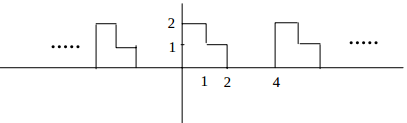
\includegraphics[width=0.7\textwidth]{figs/c1p3e1.png}
\label{fig:c1p3e1}
\end{figure} 

\item The function:
\begin{figure}[H]
\caption*{}
\centering
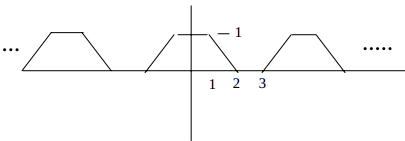
\includegraphics[width=0.7\textwidth]{figs/c1p3e2.png}
\label{fig:c1p3e2}
\end{figure} 

\end{enumerate} 

\subsection*{Solution}

Lets recall from \cite{kamen2000fundamentals} that:
\begin{equation*}
x(t) = a_0 + \displaystyle\sum_{k=1}^{\infty} A_k \cos(k \omega_0 t + \theta_k) \;
-\infty < t < \infty 
\end{equation*} 

\begin{equation}
\begin{aligned}
X_0 = a_0 \\
|X_n| &= \frac{1}{2} A_k \; , k=1,2,.. \\
\angle X_n &= \theta_k \; , k=1,2,..
\label{eq:c1p31}
\end{aligned}
\end{equation} 

\begin{enumerate}
\item 
From (\ref{eq:c1p31}) we can immediately calculate the $X_n$ coefficients:
\zcodemat{sources/c1p3a.m}{Plot Magnitude and Angle of $X_n$}

\begin{figure}[H]
\caption{Magnitude and Angle of $X_n$}
\centering
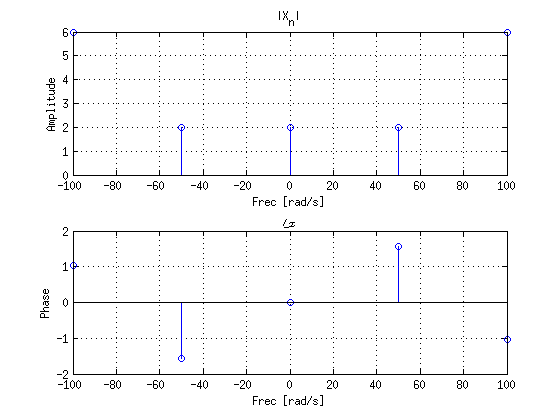
\includegraphics[width=0.8\textwidth]{figs/c1p3a.png}
\label{fig:c1p3a}
\end{figure} 

\end{enumerate} 
